% !TeX root = ./thesis.tex
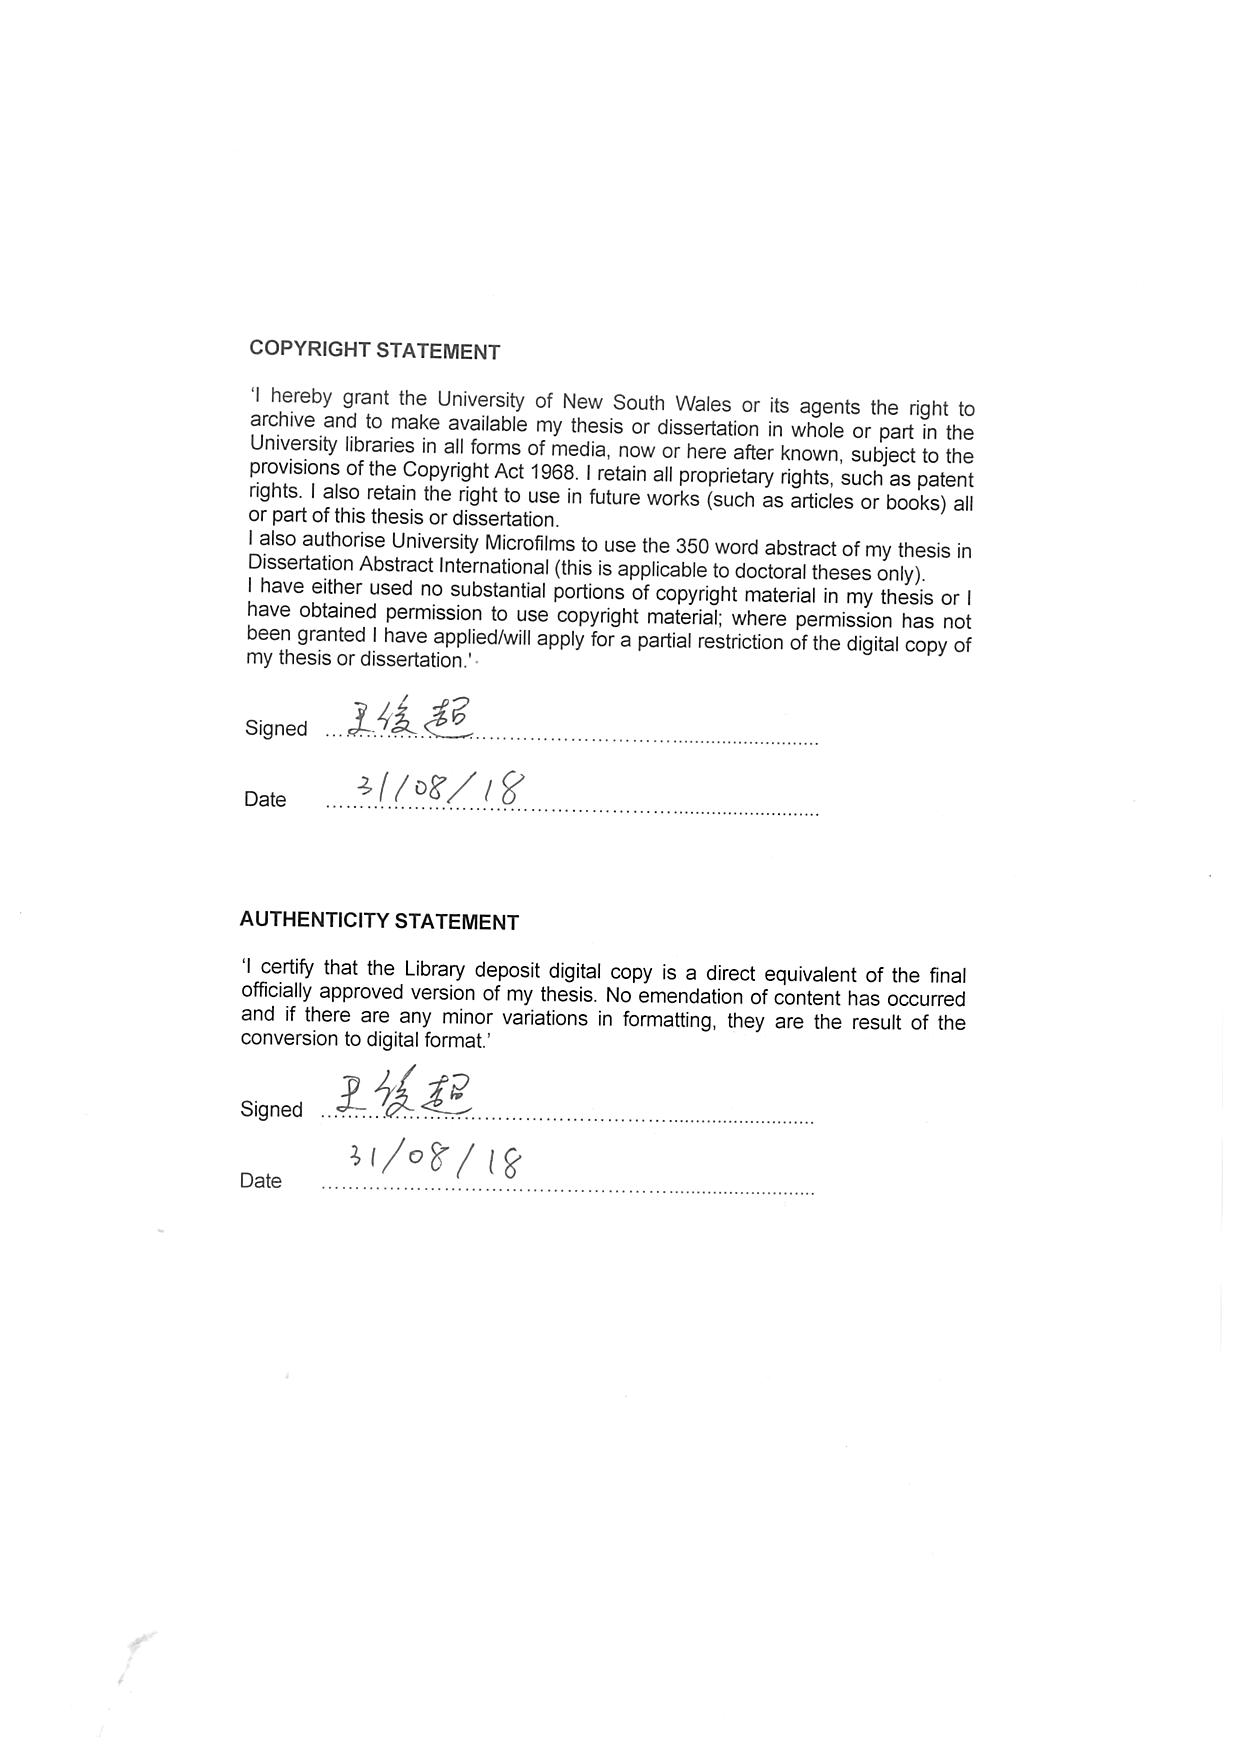
\includepdf[pages=-]{static/copyrightauthenticitystatements_signed.pdf}
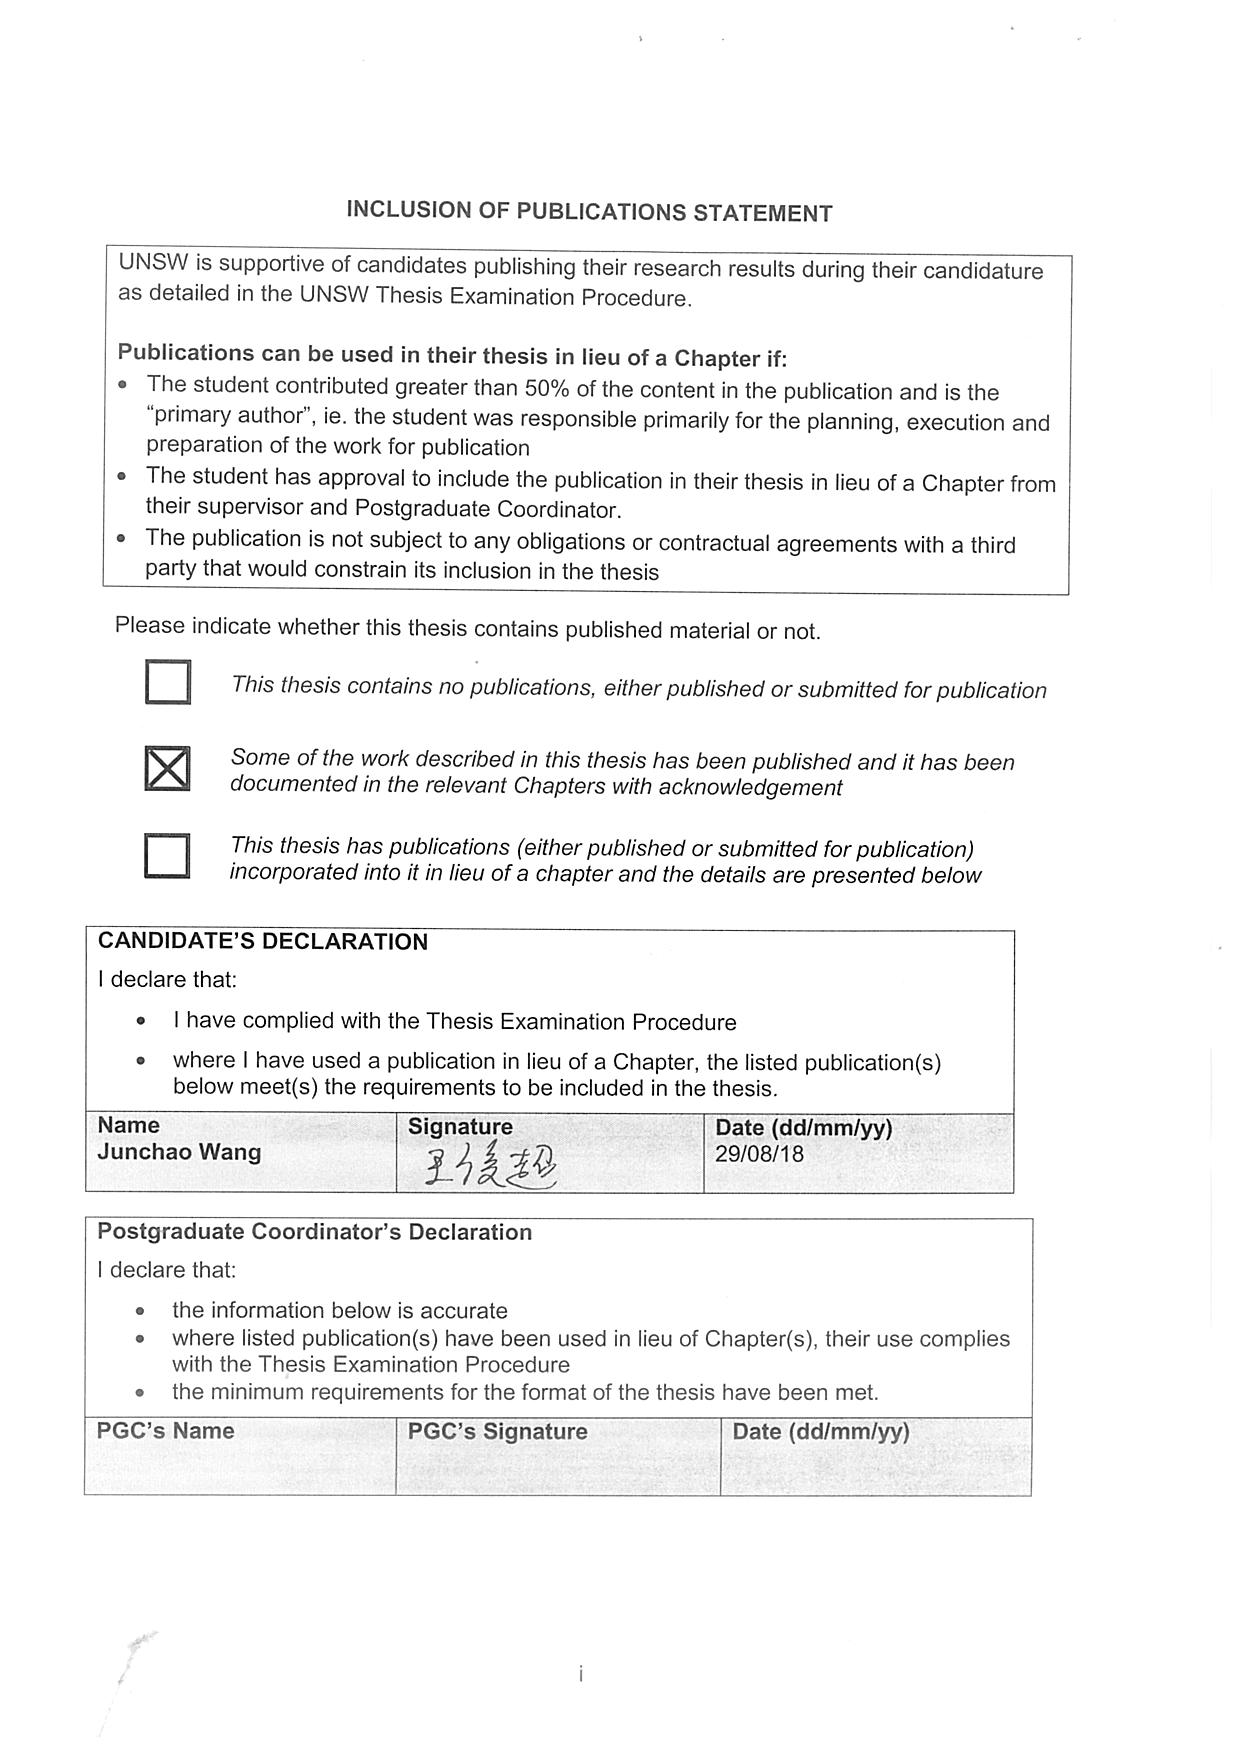
\includepdf[pages=-]{static/Inclusion_of_publications_statement_signed.pdf}
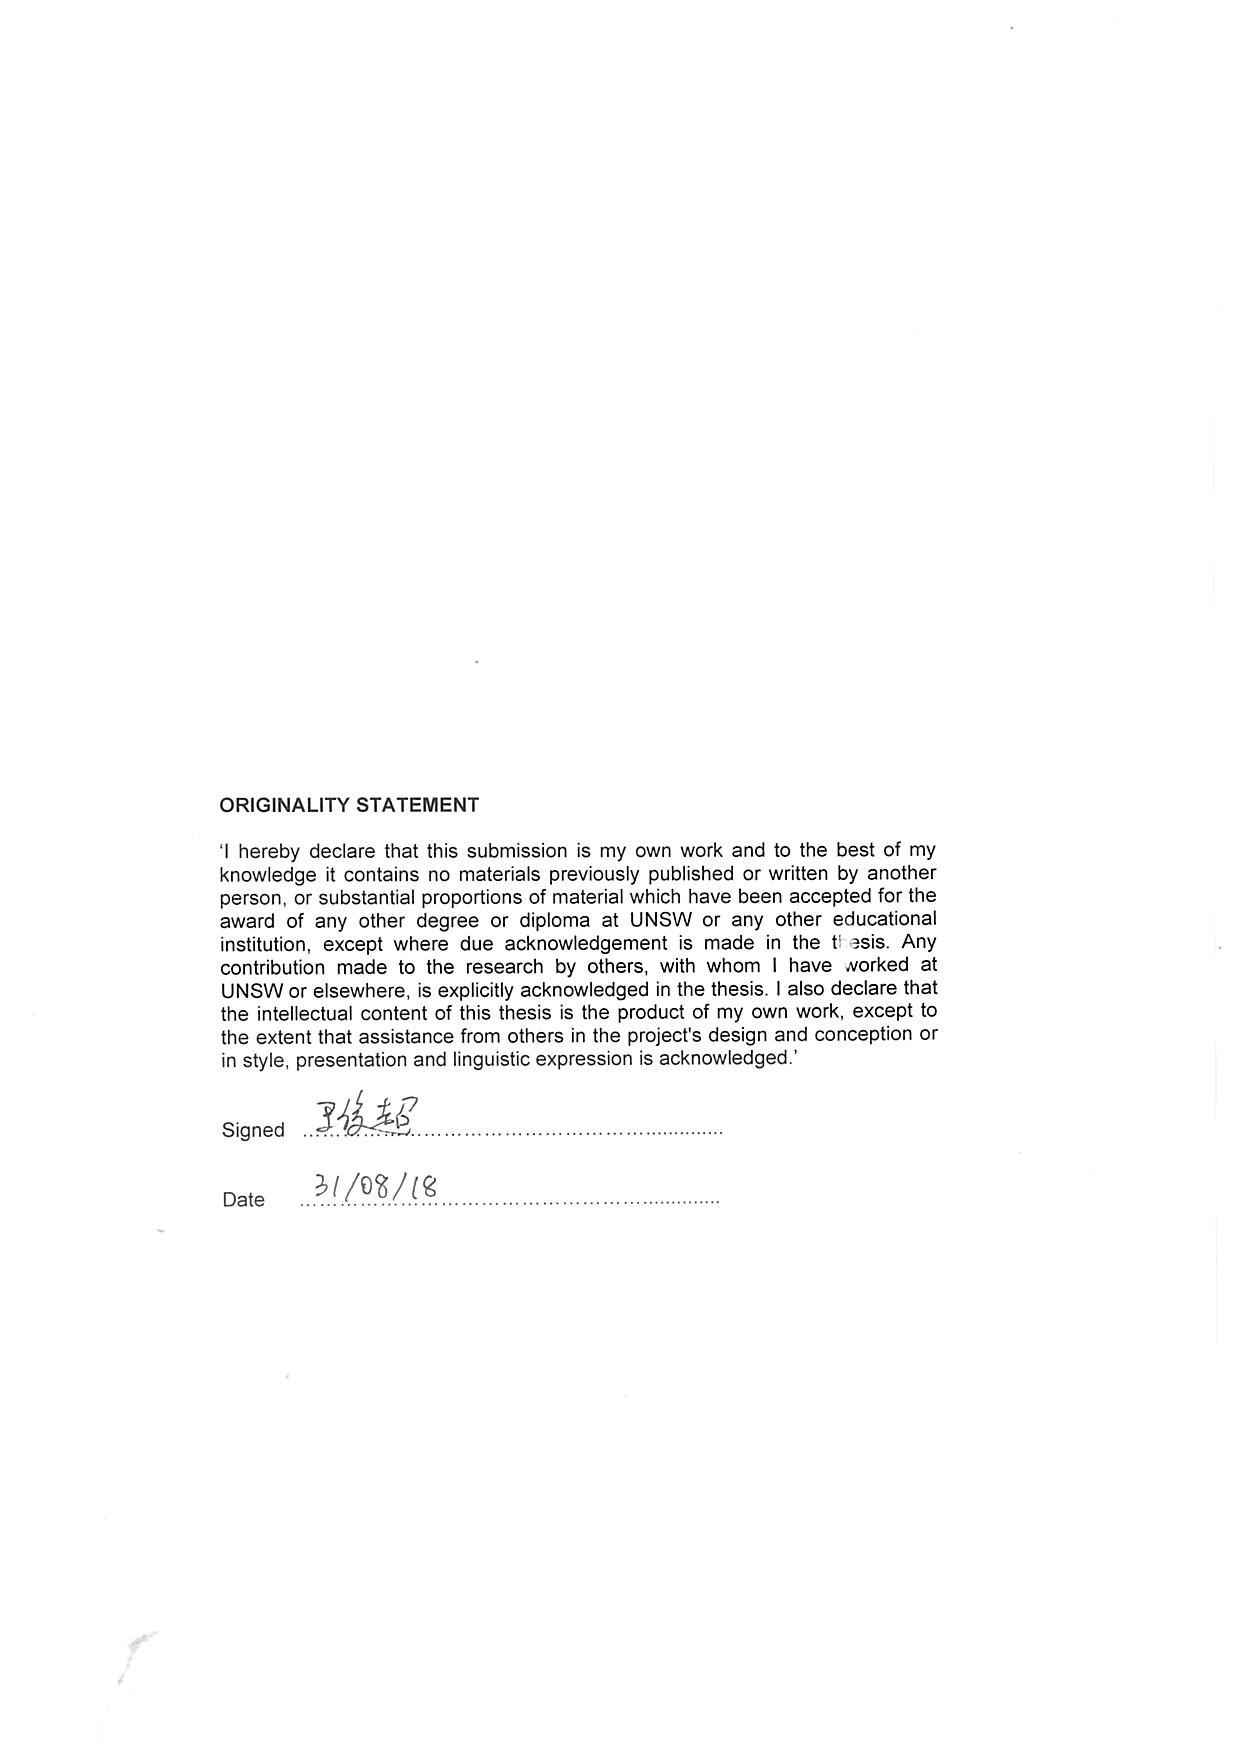
\includepdf[pages=-]{static/originalitystatement_signed.pdf}

\chapter*{Acknowledgement}
\addcontentsline{toc}{chapter}{Acknowledgement}
\paragraph{}
Foremost, I would like to express my sincere gratitude to my supervisor Prof. Chongmin Song and Dr.Sundararajan Natarajan for the continuous support of my research, for their patience, motivation, enthusiasm, and immense knowledge.
their guidance helped me in all the time of research and writing of this thesis.
I could not have imagined having a better advisor and mentor for my Ph. D Thesis.

% ------------------------------------------------------------- %

\chapter*{Abstract}
\addcontentsline{toc}{chapter}{Abstract}
\paragraph{}
The Finite element method (FEM) constitutes a general tool for the numerical solution of partial differential equations in engineering and applied science.
Great amount of research has been conducted on FEM in terms of mathematics and applications, contributing to its dominance over numerical method in solid mechanics and structural analysis.
Although it is a principle method for solving complex problems in the engineering field, deficiency in geometric representation has been detected.
Besides, it could be expensive in terms of time and human resource to create the mesh required by the FEM.
The research towards integrating geometry and analysis has led to the ‘Isogeometric Analysis’ (IGA) (Hughes et al., 2005).
However, as the CAD model provides information only of the boundary, a 2D/3D stress analysis is still one major step away.

\paragraph{}
This thesis presents a simple and efficient technique based on the combination of the scales boundary finite element method (SBFEM), automatic mesh generation and adaptive refinement algorithms to reduce the human efforts in the structural analysis.
In the SBFEM, only the boundary information is required and hence a seamless integration can be provided with the CAD modelling.
The NURBS basis functions are adopted to discretize the unknown fields in the circumferential direction within the proposed framework, whilst analytical solution is sought in the radial direction.
This framework will also be further extended to problems with singularities and to dynamic analysis.

\paragraph{}
To mode problems with complex geometries, the problems domains are divided into a mesh of scaled boundary finite elements.
A quad-tree based mesh generation algorithm is developed. High quality mesh will be generated with the help of the algorithm and the computational cost will also be improved due to the utilization of the patterns in the quad-tree.
Furthermore, no human efforts are required for the pre-processing as the output of the CAD software (i.e. IGES file) will be used to determine the geometric information automatically.
Any mismatch between the geometric representation in design and in numerical analysis may be prevented as the design is used directly.

\paragraph{}
To ensure a controllable accuracy and minimal computational cost, an adaptive and robust mesh refinement algorithm is also developed to prevent unnecessary refinement in the region which contributes little to the improvement to the accuracy.
The expressions related to the eigenvalues of the SBFEM formulation representing the quantity of the error in the interpolation are adopted as one of the error indicators, together with the area and other geometric properties of the Scaled Boundary Finite Element.
A machine learning model using the Multilayer Perceptron (MLP) is trained to determine whether a Scaled Boundary Finite Element needs refinement or not based on all these information.

\paragraph{}
The proposed method is further extended to 3D with an initial mesh generated based on the STL file and octree algorithm.
The octree mesh provides a high quality mesh in 3D for SBFEM and the IGES file from the CAD software will be adopted in order to map intersection points back to NURBS surfaces to preserve an exact geometry.
The convex hull properties of the NURBS are utilized to accelerate the algorithm.

\paragraph{}
Numerical examples are presented to verify the proposed technique with the results from the literature and the numerical results obtained using the commercial software ANSYS.
The accuracy and the convergence properties of the proposed method are demonstrated with benchmark problems in the context of linear elasticity and linear elastic fracture mechanics.
The presented results show a higher accuracy and rate of convergence of the proposed method.

% ------------------------------------------------------------- %

\chapter*{Publications}
\section*{Journal papers}
\begin{enumerate}
    \item Sundararajan Natarajan, \textbf{JunChao Wang} , Chongmin Song , Carolin Birk (2015).
    Isogeometric analysis enhanced by the scaled boundary finite element method.
    \textit{Computer Methods in Applied Mechanics and Engineering}, 283:733-762
    \item Yan Liu , Albert A. Saputra, \textbf{Junchao Wang}, Francis Tin-Loi, Chongmin Song (2017).
    Automatic polyhedral mesh generation and scaled boundary finite element analysis of STL models.
    \textit{Computer Methods in Applied Mechanics and Engineering}, 313:106-132
\end{enumerate}

% ------------------------------------------------------------- %

\chapter*{Nomenclature}
\addcontentsline{toc}{chapter}{Nomenclature}
\renewcommand{\arraystretch}{2}
\begin{table}[h!]
\begin{tabular}{lr}
    {\it Greek Letters}     &   \\
    $\epsilon$              &   Threshold   \\
    $\{ \epsilon \}$        &   Strain tensor   \\
    $\zeta(x)$              &   Softplus function   \\
    $\kappa$                &   Kolosov constants   \\
    $\lambda$               &   Eigenvalue  \\
    $\nu$                   &   Poisson's ratio \\
    $( \xi, \eta, \zeta )$  &   Scaled boundary finite element coordinates  \\
    $\{ \Xi \}$             &   NURBS knot vector   \\
    $\rho$                  &   Density \\
    $\sigma$                &   Logistic sigmoid    \\
    $\{ \sigma \}$          &   Stress tensor   \\
    $\{ \Phi \}$            &   Surface tractions   \\
    $\{ \psi_\sigma \}$     &   Stress mode \\
\end{tabular}
\end{table}
\pagebreak
\renewcommand{\arraystretch}{1.4}

\begin{longtable}{lr}
    % \begin{tabular}{lr}
        {\it Latin Letters}                 &   \\
        $\{B\}$                             &   Minibatch   \\
        $\{c\}$                             &   Integrating constants   \\
        $\{C(u)\}$                          &   NURBS curve \\
        $E$                                 &   Young's modulus \\
        $E_{a \sim b}$                      &   Cross entropy between data set $a$ and $b$  \\
        $[E_0], [E_1], [E_2]$               &   Element coefficient matrices    \\
        $\{F\}$                             &   Nodal forces    \\
        $G$                                 &   Shear modulus   \\
        $J(\theta)$                         &   Cost function   \\
        $|J|$                               &   Determinant of Jacobian matrix  \\
        $[J(\xi, \eta, \zeta)]$             &   Jacobian matrix \\
        $K_{\mathrm{I}}, K_{\mathrm{II}}$   &   Stress intensity factors for mode $\mathrm{I}$ and $\mathrm{II}$    \\
        $[K]$                               &   Stiffness matrix    \\
        $L(x, y, \theta)$                   &   Pre-example Loss function   \\
        $[L]$                               &   Linear differential operator    \\
        $[N(\eta)]$                         &   Shape function  \\
        $p$                                 &   Order of the shape function \\
        $[P]$                               &   NURBS control points    \\
        $\{q(\xi)\}$                        &   Internal force vector   \\
        $(r, \theta)$                       &   Polar coordinates   \\
        ${S(u, v)}$                         &   NURBS surface   \\
        $\{ u \}$                           &   Displacement vector \\
        $[w]$                               &   NURBS surface weight matrix \\
        $\{w\}$                             &   NURBS curve weight vector   \\
        $(x,y)$                             &   Nodal coordinates   \\
        $[Z]$                               &   Hamiltonian coefficient matrix  \\
    % \end{tabular}
\end{longtable}

\renewcommand{\arraystretch}{1}
% ------------------------------------------------------------- %

\tableofcontents
\listoftables
\addcontentsline{toc}{chapter}{List of Tables}
\listoffigures
\addcontentsline{toc}{chapter}{List of Figures}